\chapter{ユーザ調査}
本章においては,本研究の動機にもなった,アプリケーションユーザが入力として用いたい手書きジェスチャの調査内容とその結果について述べる.

\section{アプリケーションユーザへの手書きジェスチャの調査}
単一ストロークからなる手書きジェスチャ認識を用いたシステムが,これまでにも多く開発されてきた.その中で,\$1は,  ~\cite{Hong:2000:STI:354401.354412, Landay:1993:EEU:259964.260123, Lin:2000:DFT:332040.332486}において用いられているような,一般的にスマートフォンやタブレット端末などのタッチパネルへの手書き入力やペン入力において良く用いられる,単一ストロークからなるジェスチャを抜粋し~(図\ref{fig:stroke_1}),それらについて認識率を計測した.\TODO{それぞれについて詳しく書く.}
しかしながら,ユーザ定義ジェスチャを用いた研究~\cite{Vatavu:2012:UGF:2325616.2325626, Bragdon:2011:EAT:1978942.1979000, Wobbrock:2009:UGS:1518701.1518866, Shimon:2015:EUB:2785830.2785890}の中には,単一ストロークからなるジェスチャであり,かつ,ストロークの形状は同じであるが,ストロークの向きや位置の違いを利用したジェスチャを入力に用いる場合があった.

そこで,普段スマートフォンを利用する場面,およびスマートフォンを入力デバイスとしPCを操作する場面を想定した時,どのようなアプリケーションに対し,どのような手書きジェスチャを入力として用いたいかを事前調査した.

\begin{figure}[!h]
\centering
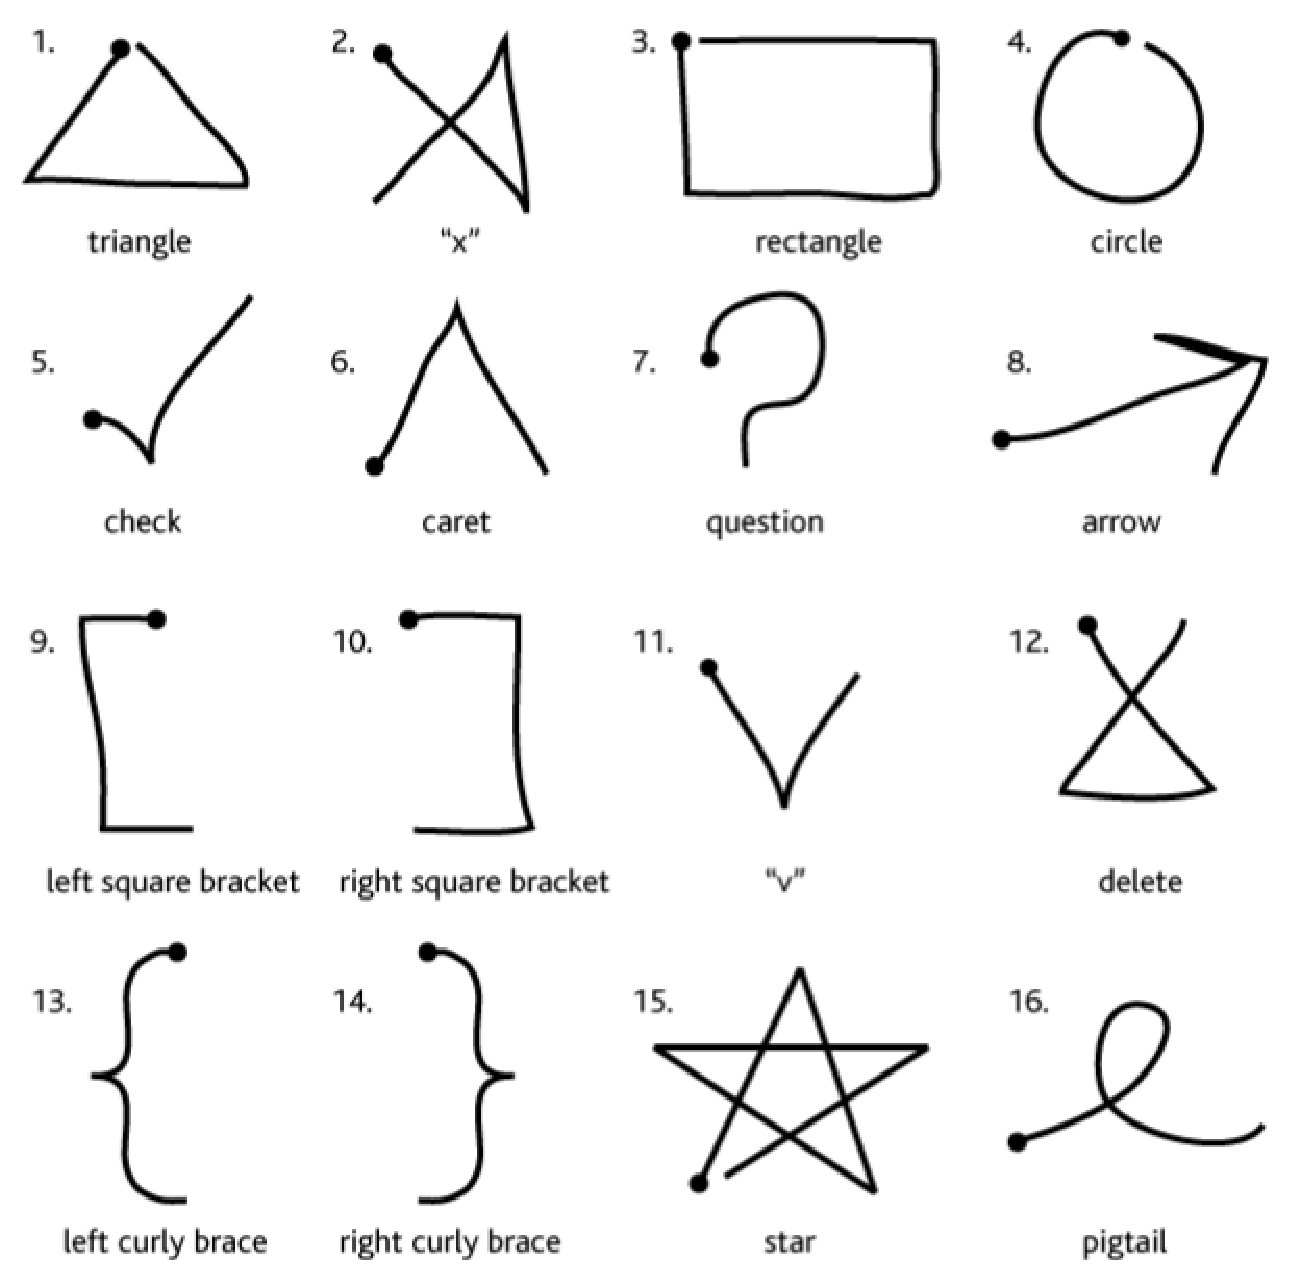
\includegraphics[width=0.4\columnwidth]{img/stroke_1.eps}
\caption{\$1において用いられる,一般的にスマートフォンやタブレット端末などのタッチパネルへの手書き入力やペン入力において良く用いられる,単一ストロークからなる手書きジェスチャの例}
\label{fig:stroke_1}
\end{figure}

\section{被験者}
被験者は普段からスマートフォンを使用している大学院生の男性6名である.年齢は21〜27歳~(平均23.8歳)であり,全員右利きであった.6名の被験者の中にはコンピュータサイエンスあるいはユーザインタフェースを専攻している人が4名存在し,残りの2名は,社会工学を専攻している男性と,エンジニアとして働いている男性であった.被験者は全員日頃からスマートフォンを使用していた.

%\section{調査に用いた機器}
%実験には,入力端末であるスマートフォンとしてiPhone5を用い,実験における入力領域は1.94'' × 3.18''であり,解像度は640 × 1036である~(図\ref{{fig:screenshot}}).

 %\begin{figure}[!h]
%\centering
%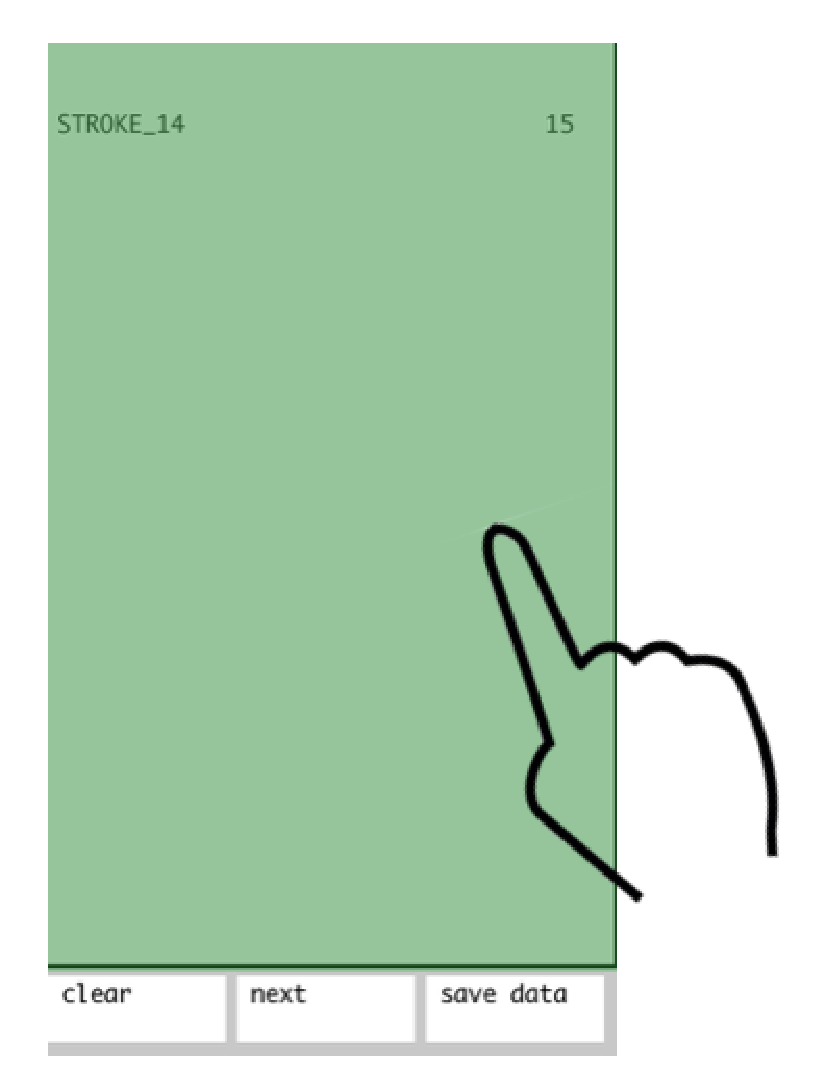
\includegraphics[width=0.4\columnwidth]{img/screenshot.eps}
%\caption{The screen shot on the smartphone. The green area is the input area}
%\label{fig:screenshot}
%\end{figure}

\section{調査手順}
%教示を詳しく書く
%使いたいジェスチャを入力することを示す
我々はまず,被験者に調査の目的を説明した.
その後,普段スマートフォンを利用する場面,およびスマートフォンを入力デバイスとしPCを操作する場面を想定した時,どのようなアプリケーションに対し,どのような手書きジェスチャを入力として用いたいかを20以上考えるよう指示し,自身のスマートフォンに対し実際に入力しながら考えるよう指示した.
%図\ref{fig:screenshot}における緑色の領域部分にジェスチャを入力するよう指示した.
その際,ジェスチャを入力する姿勢は次の3つの姿勢~(姿勢1,姿勢2,姿勢3)から,実際に自分がそのジェスチャを入力として用いるときに入力する姿勢として1つ選んでもらった.
\begin{enumerate}
\item 机にスマートフォンをおいて,利き手の人差し指によって入力する.
\item 利き手でスマートフォンを握りながら,同じ利き手の親指によって入力する.
\item 利き手とは反対の手でスマートフォンを握りながら,利き手の人差し指によって入力する.
\end{enumerate}
被験者は,全ての姿勢を座って入力するよう指示された.
また,入力ジェスチャとして,単一ストロークからなるよう指示した.

入力として用いたい手書きジェスチャを1つ考えるたびに,我々は付録\TODO{何の付録か}に示す紙にそのジェスチャをボールペンによって書くよう指示した.またそれに加え,そのジェスチャを入力した姿勢~(1〜3),そのジェスチャをどのアプリケーションに対して用いたいのかも同時に書くよう指示した.


\section{調査結果}
図\ref{fig:elicetated_strokes}は,6人の被験者から得られた手書きジェスチャ一覧である.

図\ref{fig:elicetated_strokes}において,例えば音楽再生アプリケーションにおいて,早送り,巻き戻し,音量の上げ下げ,といったような前後への移動や,値の上げ下げなど,対になるような操作に対して,向きや大きさの違いを用いて入力する要望があった.また,ブラウザアプリケーションにおいて,位置によって登録先のブックマークを変える,ページ内における表示位置をジェスチャの入力位置に対応させる,といったように,位置の違いを操作対象先の違いに割り当てたり,現在操作しているものの位置に対応付けるといった要望があることがわかった.

また,片手で操作する場面~(姿勢2)においては,難しいストローク操作ができないため,極力簡単なストロークを用い,かつ,大きさ,向き,位置の特徴量を利用して入力する要望があることも分かった.
\TODO{ここら辺もうちょい詳しく書く?}

\begin{figure*} [t]
 \begin{center}
  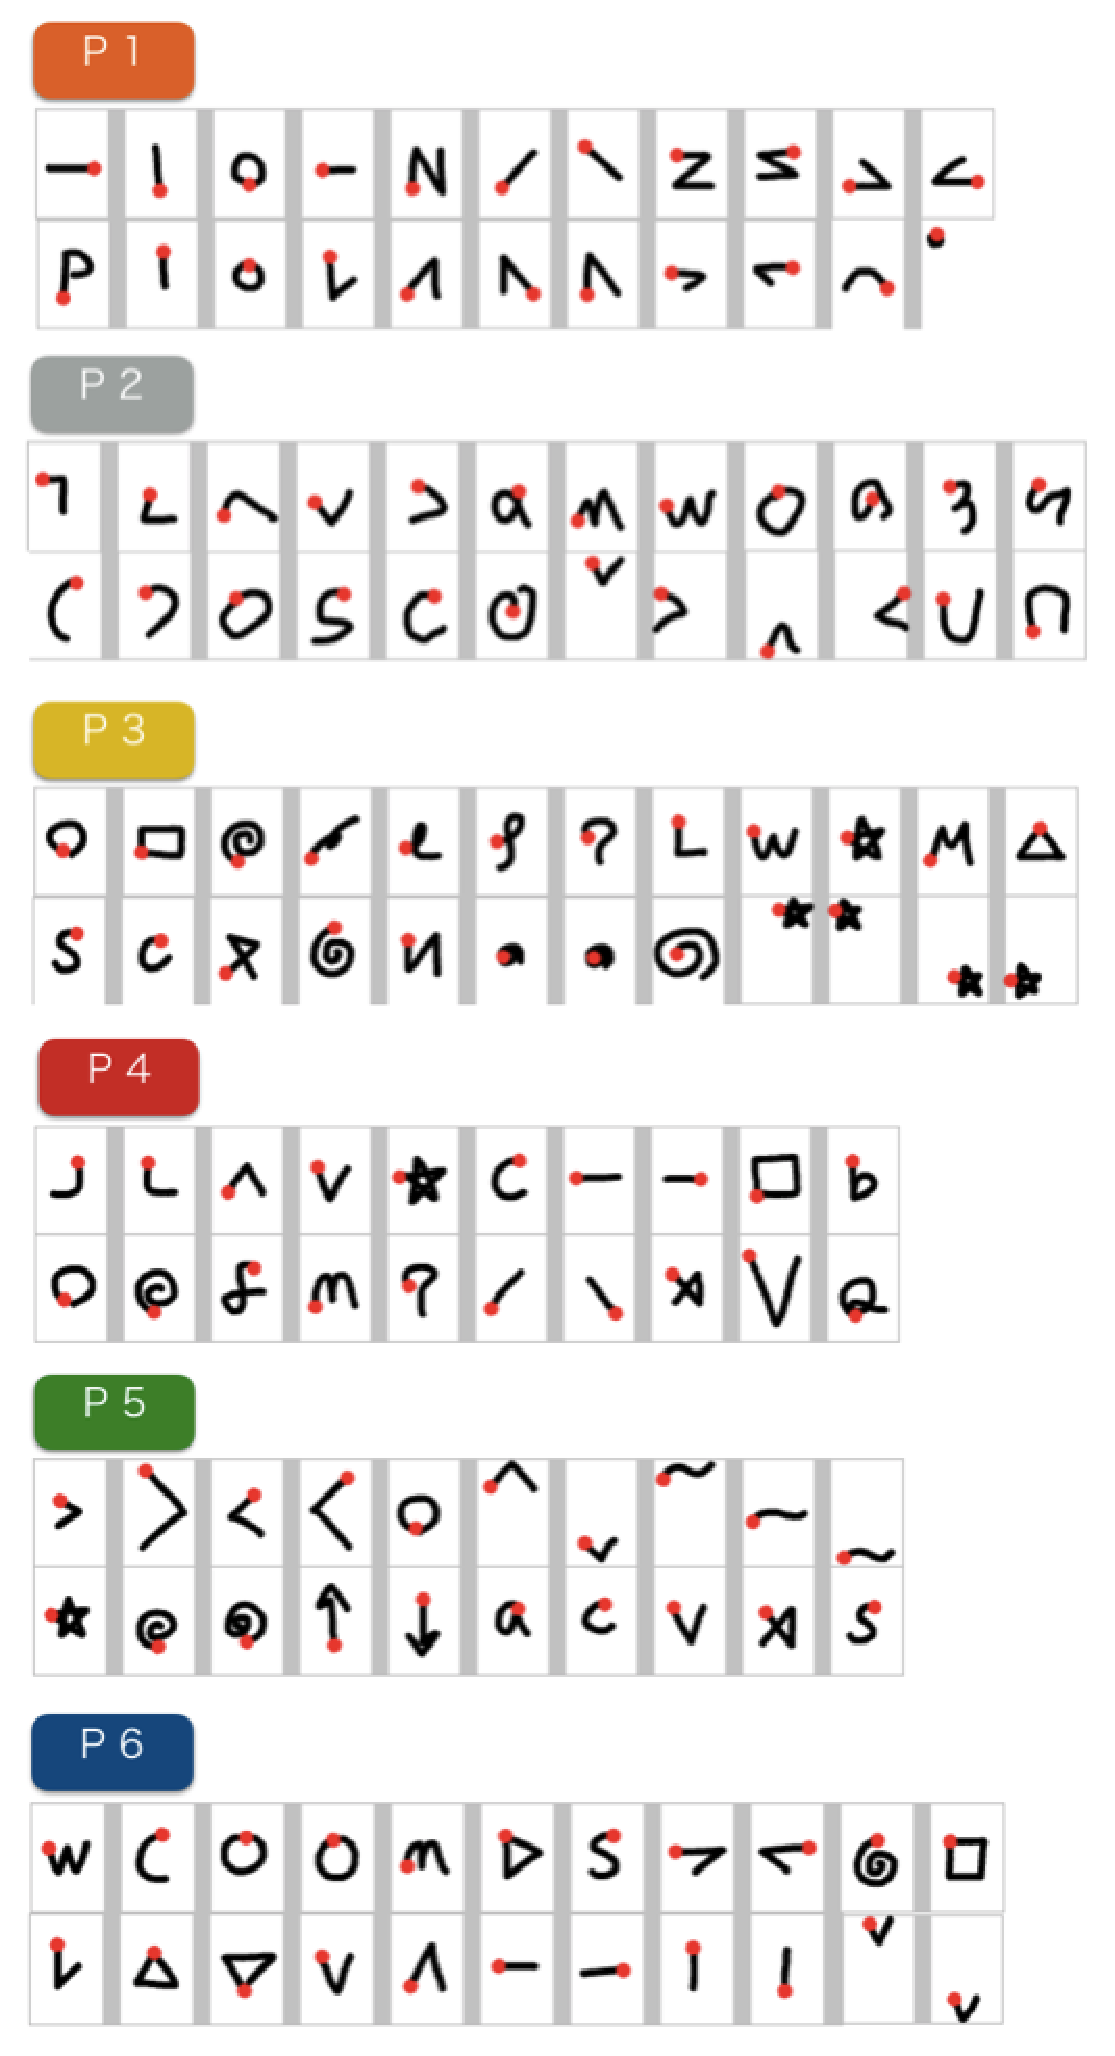
\includegraphics [width=0.7\columnwidth]{img/elicetated_strokes.eps}
  \caption{調査において6人の被験者~(P1〜P6)から得られた,用いたい手書きジェスチャの一覧}
  \label{fig:elicetated_strokes}
 \end{center}
\end{figure*}

\$Vは,図\ref{fig:elicetated_strokes}が示すような,ジェスチャの形状や書き順は同じでも,大きさ,向き,位置に関して異なる手書きジェスチャを認識することが可能なアルゴリズムであり,今回調査を行った被験者の要望を満たすことのできる手書きジェスチャ認識である.


%\$Vは,\$1にアルゴリズムを少し追加するだけで,\$1が示す認識率と認識速度を維持しつつ,図が示すような,ジェスチャの形状は同じでも,大きさ,向き,位置に関して異なるジェスチャ認識アルゴリズムである.




